\chapter{Background \& Literature Review}
	\label{chap:background_lit_review}
	
	To be able to implement our application, with the desired outcomes, we must first look into several key topics backgrounds. First, we will be looking into educational games, and what makes something an educational game. Then we will be looking into a motivational feature called gamification and how it is used in education and within greater science concepts. As well as the different types of machine learning models and different ways these models are currently getting taught to potential students.
	
	We wanted to find out what the context of gaming and what gamification is, and how it can be used within education, to take aspects of teaching and learning that can get brought into the 21st Century. To make aspects of education more accessible to students in a manner that they are more accustomed to in their everyday lives. 
	
	\section{Introduction to Educatiuonal Games}
		\label{sec:intro_to_edu_games}
	
	Games that get designed with educational purposes as its intention, or that have incidental or a secondary educational value get categorised as educational games. Although` all types of games can get used within an educational setting. However, only games that get designed to help learners learn about certain subjects, expand concepts, reinforce development, understand a historical event or culture, or assist them in learning a skill as they play can get classed as an educational game. Game types include board, card, and video games. As educators, governments, and parents realise the psychological need and benefits that gaming has on learning, this educational tool has become mainstream \cite{barab2009transformational}. 
	
	Research suggests that there are three main approaches to creating software that stimulates cognitive growth within a gamer. These are building games from scratch that have been created by educators and programmers, integrating commercial off-the-shelf games and finally creating games from scratch, which have been done by the students \cite{van2006digital}. For these to work these approaches requires the teacher to buy into the positive results of using digital games for education. It also requires teachers to have adequate self-efficacy concerning the use of these games and their technology. The students usually have high amounts of self-efficacy in the usage of digital games. In contrast, the lack of confidence teachers have in incorporating digital games usually results in the delivery of less effective educational use of the games. However, Gerber and Price have found that teachers' inexperience with digital games does not prevent them from the desire to incorporate them in-class instruction \cite{gerber2013fighting}.
	
	
	\subsection{Gamification}
	%%% From HCI Report
	Gamification, a term first coined in 2002, is an HCI technique used to add a game layer to traditional non-game like situations. Gamification aims to create extrinsic motivators for a person to be encouraged to do particular actions. Each action, upon completion, will have a little reward which, upon doing so, will release dopamine into the brain. The release of dopamine creates a good feeling within the participant's mind, which in turn encourages them to do it again. These rewards can be in the form of badges, achievements or progress bars, to name a few.
	
	The term gamification first appeared in the context of software design in 2008 \cite{4}, but the term got more widespread recognition within 2010. However, the term "gamification" was first coined by Nick Pelling in 2002 \cite{3e}. His initial aim with gamification was to combine the social and rewarding features of games into the software. Gamification started to gain much attention, so much so that it got described as one of the most promising areas of gaming \cite{5}. Gamification is now known as a powerful tool for engagement, which has, since its initial conception, now becoming a conventional feature within software development \cite{3e}. Researchers consider gamification to be the progression of earlier work that focuses on adopting game-design elements to non-game situations and contexts. Research in the HCI field, in regards to apps that use game-driven components for motivation and also in interface design, suggest that there is a connection between Soviet concepts of socialist competition and the American management trend of "fun at work" \cite{5}.
	
	Jane McGonigal, in 2010, delivered a groundbreaking TED Talk titled, "Gaming Can Make a Better World' \cite{6}. This talk is known as the defining moment in the history of gamification. During the talk, she foresees a game based paradise as she states within her talk "I know two things for sure: that we can make any future we can imagine, and we can play any games we want, so I say: Let the world-changing games begin \cite{6}." Hindsight shows she was correct, as, from 2011, gamification starts to pick up steam.  At a Computer-Human Interaction (CHI) conference, a workshop titled "Gamification: Using Game Design Elements in Non-Gaming Contexts \cite{7}", which in the year of 2011 created the Gamification Research Network (GRN) \cite{11}. Through the following years, gamification continues to grow. Gamification goes viral without people knowing through a game called Pokémon Go where it became one of the most successful applications of gamification ever, with over 800 million downloads. People who would usually turn their nose up at badge collecting were out walking the streets searching for rare Pokémon. Pokémon Go is one of the most successful apps of all time, so much, so it even broke records \cite{3e,8}. It could be said thanks to Pokémon Go, that gamification is now everywhere.  
	
	%%%%%%%
	
	
	\subsection{Gamification in Education}
	%%% Taken from HCI report
	The gamification within a learning setting is a pedagogical approach to motivate students. This approach tried to help students learn by using gaming elements within a learning environment \cite{22}. Gamification within education is very much the same thing, in general, as gamification. However, within education, it has a focus on aiding learning instead. Gamification in learning has two main views. One of the views categories gamification of learning as learning which has game-like characteristics. However, this view believes it is only the case when only when the learning is happening in a non-game setting, like a classroom. This view would involve a range of elements that get presented in a  game layer which attempts to happen alongside the learning in a traditional classroom. The other view has the same views as the view just mentioned, but the other half also include games that get designed to provoke learning within them \cite{22}. 
	
	Gamification, within an educational or a learning situation, has many benefits. While traditionally gamification has been used to improve attendance with incentives by reaching a set score or receiving extra prizes for completing designated tasks within a lesson. It can also aid in cognitive development within youngsters, which can boost levels of engagement and can assist with accessibility within the classroom \cite{24}. Games that get created for improving cognitive development are known as "brain games" \cite{24}. These popular games typically are focused around a series of questions and problems to solve or answer. These games develop the rate the player can sustain information and increase the brain's ability to process knowledge. The levels of the engagement increases when gamification has gets used within a classroom \cite{25}. A study performed by scientists aimed to measure the students' levels of engagement in a classroom where gamification elements are applied \cite{25}. They assigned a point system to multiple daily activities, and every student had a measurement of their observed level of engagement. The finding showed that the game like setting was supporting the learning within the classroom and increased productivity. Therefore, by increasing engagement levels, it also means it helps students be able to access the content of the lesson better. 
	
	Gamification of learning has excellent potential benefits. The gains allow students to have ownership of their education, as well as giving opportunities for the learner to gain a sense of their "own identity" through alternative role-playing selves. The freedom that gets bundled without any negative repercussions allows the students to fail and keep on trying again. The ability to increase fun and joy while learning. The opportunity for tasks to be differentiated. Making the learning visible and providing opportunities to inspire intrinsic motivators for learning. Also, the ability to aiding in motivating students with low levels of motivation \cite{22}. 
	
	Even though gamification can aid teaching students of all needs, a study conducted on students who had autism using video games showed that this training method was powerful in teaching the content that was age-appropriate \cite{26}. However, gamification of learning is not something just for the classroom. It is an excellent tool for learning outside the classroom and allowing education to get conducted without an educational facilitator like a teacher. 
	
	%%% Taken from CSCM10 Report
	\subsection{Gamification in Science}
	\label{sec:game_in_science}
	
	The National Research Council report argued that science is the discipline that should convey those skills required for a twenty-first-century workforce, such as non-routine problem solving, adaptability, complex communication/social skills, self-management, and systems thinking \cite{national2010exploring}. Creating a scientifically literate population requires a strong science education \cite{morris2013gaming}. This statements spawned a focus on how video games have the potential to be exploited for gain in science education.
	
	Science operates and develops at multiple spatiotemporal scales; it is simultaneously an individual and social activity that uses and creates cultural tools. We use the phrase cultural tools \cite{weiner1995attribution} to describe tools such as language, cognition, and information-seeking strategies that augment human understanding and get used in both formal, for example within classroom instruction, and informal education, for example, parent-child interactions \cite{rosas2003beyond}. Cultural tools can be conceptual, for example, teaching in critical thinking, or concrete, for example, notebooks, scientific instruments. As is the case with psychological studies of the basic cognitive mechanisms involved in reading and mathematical thinking, basic research on scientific thinking can and should inform educational practice \cite{morris2013gaming}.
	
	There are three different ways in which video games may support the development of scientific thinking and science education \cite{morris2013gaming}. First, there are some games, often referred to as serious educational games\cite{annetta2008serious}, in which scientific domain knowledge gets taught by using the gaming context to promote inquiry-based learning. An example being, Supercharged! \cite{squire2003harnessing}. This game has gotten designed to teach principles of electromagnetism. Cheng and Annetta used a video game to give students instruction on the effects of methamphetamine on the brain, and Immune Attack teaches immunology concepts \cite{cheng2012students}. These games incorporate core disciplinary ideas relating to the third dimension of the Framework for Science Education \cite{national2012framework}. Learning the wide range of discipline-specific content may be difficult to adapt to gameplay, given the vast number of possible science concepts that can get taught \cite{morris2013gaming}. These types of games get utilised by industries like scientific exploration, education, health care, defence, emergency management, city planning, engineering and politics \cite{wikiserious}. Although not all do, serious games tend to share aspects closely tied with simulational games. However, all serious games still have other gamification features included.
	
	There are games in which instruction in scientific process skills get embedded within the game. For example, River City is a multi-user virtual environment which involves small teams of students conducting scientific investigations into an epidemic which has affected a historical town \cite{galas2006river, nelson2007robust}. Mad City Mystery is another game that has got designed to teach students interrogation and argumentation skills as they examine a strange death \cite{squire2007mad}. These games relate to the scientific practices in the first dimension of the National Research Council Framework \cite{national2012framework}.
	
	Additionally, some games may promote the development of skills, attitudes, and values that are useful for scientific thinking or practice, but without any precise instruction in scientific knowledge or skills. Some of these games can insert scientific methods or support crosscutting concepts \cite{national2012framework}. They may also reinforce concepts related to science as a multi-scale, social, collaborative endeavour. For example, establishing cognition in a contextualised virtual environment, providing joint gameplay structures, and role-playing characters are elements found in many successful commercial games that could get exploited to situate gamers in the context of scientific investigation. These games may also increase working memory capacity, an essential element in problem-solving \cite{morris2013gaming}. Adachi and Willoughby report that playing strategic instead of action video games predicts higher self-reported problem-solving skills \cite{adachi2013more}. 
	
	Nonetheless, in regards to the field of science, serious games' role is to include crucial activities for scientists. These include outreach, teaching and research. With serious games on the increase, an emerging sub-genre is called citizen science games (CSGs) \cite{10seriousrules}. CSGs enables the user to produce as well as, or instead, analyse data for scientific use. Some examples of CSGs are GalaxyZoo, Foldit and HiRE-RNA \cite{follett2015analysis,mazzanti2017can}
	
	Studies suggest that there are ten main rules for serious games to follow. These are \cite{10seriousrules}: Define a serious goal - we must first define the purpose of the game at the beginning of its development. Is its purpose for science, outreach, teaching or a combination of all three? Get the balance between entertainment and serious tasks - the game design should be implemented as a function of the objectives of the game. Therefore equilibrium and compromise need to be found between scientific accuracy and player accessibility. Allow the player to interact with the scientific data - players interest increases if they can interact with the science data, enriching the learning experience. The ability for players to generate data also creates another perspective for the player, increasing interaction. Promote onboarding and engagement - Expectations of players are varied. Therefore the reward system needs to be versatile. Ideally, the entry-level should be low and the difficulty altered to each player. Manage Information Flow - How the information to the play gets received will impact their behaviour, either positively or negatively. So if the focusing is on the outcome, this could influence the results. Provide an appropriate narrative - This is important for all games, but also crucial for serious games. The story should give the player context to the game, allowing them to know what to do. Adapt the level design - Depending on the objective, variation on level designs needs implementing. These can include duration, tasks and difficulty. Develop good graphics that are not just pleasing on the eye - High-quality graphics increase the player's immersion into the game. Use all modalities, mostly sound - Using only a visual channel can overload the player. Therefore it is vital to take the load of the player's vision and use several different channels — for example, sound. Iteratively assess what works and what does not - However, it is vital to take into account three different perspectives for serious games. The developer, the player and the scientist as they all have different views on what they believe the game needs adapting based on their desires.
	
	\subsection{Example Applications}
		\label{sub_sec:example_apps}
	
	Games like Spore create a deeper understanding of life and evolution as the game simulates a world where the player's character will evolve, adapting to their surroundings through reproduction. Another game by the same creator, Will Wright, Sim City aims to teach the player key skills like \cite{27}: Supply and demand, Budgeting, Urban planning, Managing the environment, Understanding utilities and services like transport systems and public services, Reading and maths skills.
	
	Some serious educational games Supercharged! \cite{squire2003harnessing} is a game designed to teach the principles of electromagnetism. Some other examples of series games are GalaxyZoo, Foldit and HiRE-RNA.
	
	An educational game that gets used regularly by schools is My Maths.
	My Maths is an interactive maths learning that can get used for a whole school. My Maths provides complete curriculum coverage from Key Stage 1 to A-Level. MyMaths offers interactive lessons, "booster packs" for revision, and assignable homework and worksheets, along with a wealth of resources that will help you deliver your teaching in the classroom and at home to develop your students' confidence and fluency in maths \cite{my_maths}.
	
	\begin{figure}[t]
		\begin{center}
			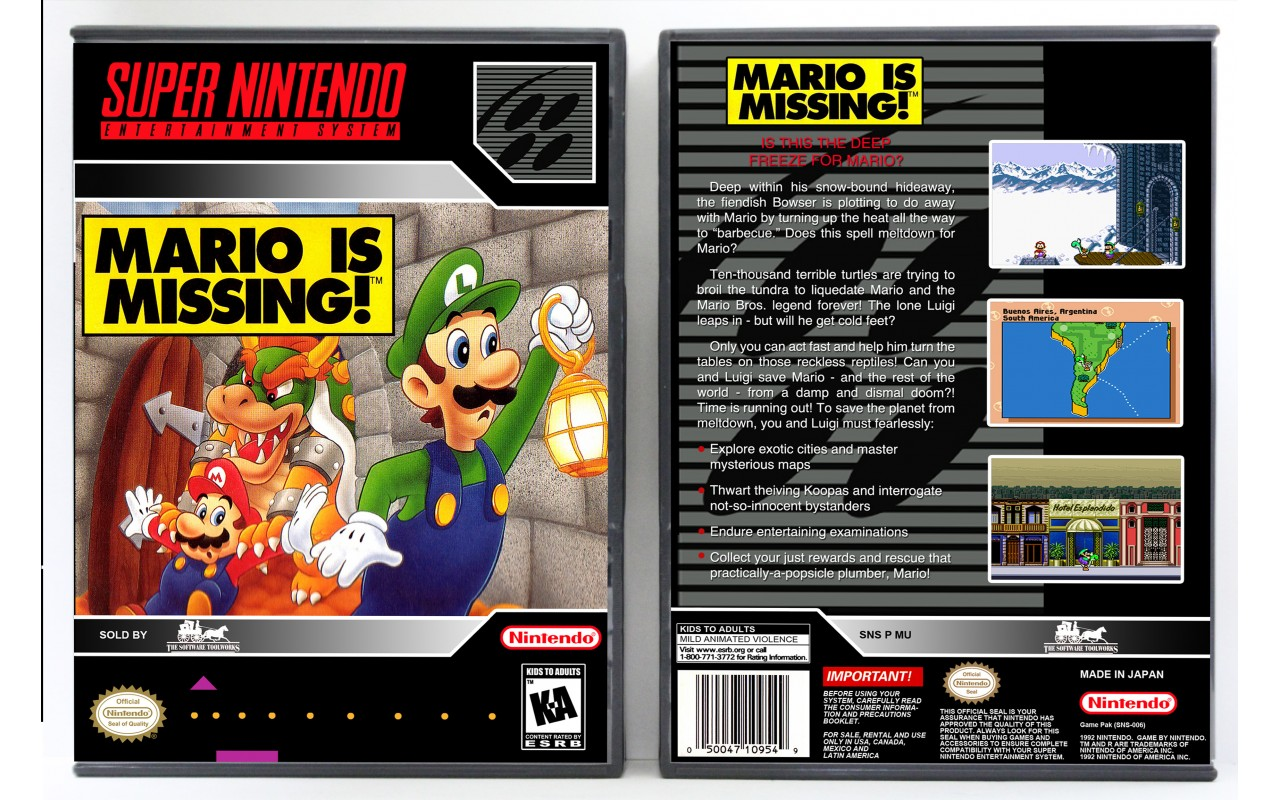
\includegraphics[width=9cm]{graphics/Mario_is_Missing_box_art.jpg}
			\caption{Box art and game discription for Mario is Missing! \cite{gaming_relics}}
			\label{fig:mario_is_missing}
		\end{center}
		
	\end{figure}
	
	Examples of educational games are Brain Training, and the Nintendo Entertainment System's Mario is Missing, both created by Nintendo.  Brain Training, also known as Dr Kawashima's Brain Training: How Old Is Your Brain?. The game features a variety of puzzles, including Stroop tests, mathematical questions, and Sudoku puzzles, which are all designed to help keep certain parts of the brain active. It has received both commercial and critical success, selling 19.01 million copies worldwide (as of March 31, 2020) \cite{bt_sales} and has received multiple awards for its quality and innovation \cite{bt_award}. Mario Is Missing! (fig: \ref{fig:mario_is_missing}) was released in 1993. The player controls Luigi, who must travel around the world to find and return stolen treasures as part of a quest to find his brother, Mario, who has been captured by Bowser. While using traditional game mechanics, that players were used to when playing Super Mario Bros., were used this allowed heuristic values to be added to let them be more of a focus on using educational challenges for the players to complete to progress.
	

	\section{Machine Learning}
	
	
	\subsection{Supervised vs Unsupervised Learning}
	%%% Spec
	Within machine learning, there are multiple different learning styles. These styles are known as supervised, unsupervised, semi-supervised and reinforcement learning. However, we will only be focusing on the main two types of techniques, supervised and unsupervised learning. 
	
	Supervised learning trains a model on known input and output data so that it can predict future outputs, and unsupervised learning, which finds hidden patterns or intrinsic structures in input data \cite{geron2019hands}. Supervised machine learning aims to build a model that makes predictions based on evidence in the presence of uncertainty. The algorithms for supervised learning takes the knowledge it has gained from a known set of input data and known responses to the data (output). These known responses are also known as labels. The combination of the labels and the data helps train the model to generate reasonable predictions for the answer to new data getting presented to the model \cite{matlanintrotoml, geron2019hands}. 
	
	Supervised learning uses classification, like neural networks, k-Nearest Neighbours, Support Vector Machines, and regression techniques, like logistic and linear regression, to develop predictive models.  Classification is a technique that predicts discrete responses by aiming to classify the inputted data into different classes \cite{matlanintrotoml}. Some examples of this type of these methods are deciding if an email is spam or not, or deciding if a patient has a benign or cancerous tumour. These types of applications also included credit scoring, medical imaging and speech recognition. While supervised learnings other method, regression techniques, aims to predict continuous responses \cite{geron2019hands}. An excellent example of this is checking for changes in the temperature or for checking the power demands fluctuations and forecasting electricity load. These kinds of applications can also get used for trading  \cite{matlanintrotoml}.
	
	The other primary method learning, unsupervised learning, aims to find hidden patterns or intrinsic structures in the data \cite{geron2019hands}. In the same regard as supervised learning, unsupervised learning seeks to obtain insights from the data. However, where supervised learning has the output labels for the provided dataset, unsupervised does not. So unsupervised learning aims to explore the data to find patterns or groupings in the data \cite{matlanintrotoml}. Unsupervised learning can take the form of clustering, like k-means, GMM, or through a technique called association rule. Examples of clustering applications include gene sequence analysis, market research, and object recognition and examples of the association rule are services providing a recommendation, like Netflix's "watch next" or Amazon's "you might also like" \cite{matlanintrotoml}.
	
	
	\subsection{Machine Learning Models}
	
	\subsubsection{K-Means}
	The KMeans algorithm aims to clusters the data by trying to separate samples into $n$ groups of equal variance (see fig: \ref{fig:km_handson_example}). While also seeking to minimise a criterion known as the inertia or even referenced as a within-cluster sum-of-squares \cite{geron2019hands, sklearn_km}. The formula for the sum-of-squares is \cite{sklearn_km}: $\sum_{i=0}^{n}\min_{\mu_j \in C}(||x_i - \mu_j||^2)$. 
	
	\begin{figure}[t]
		\begin{center}
			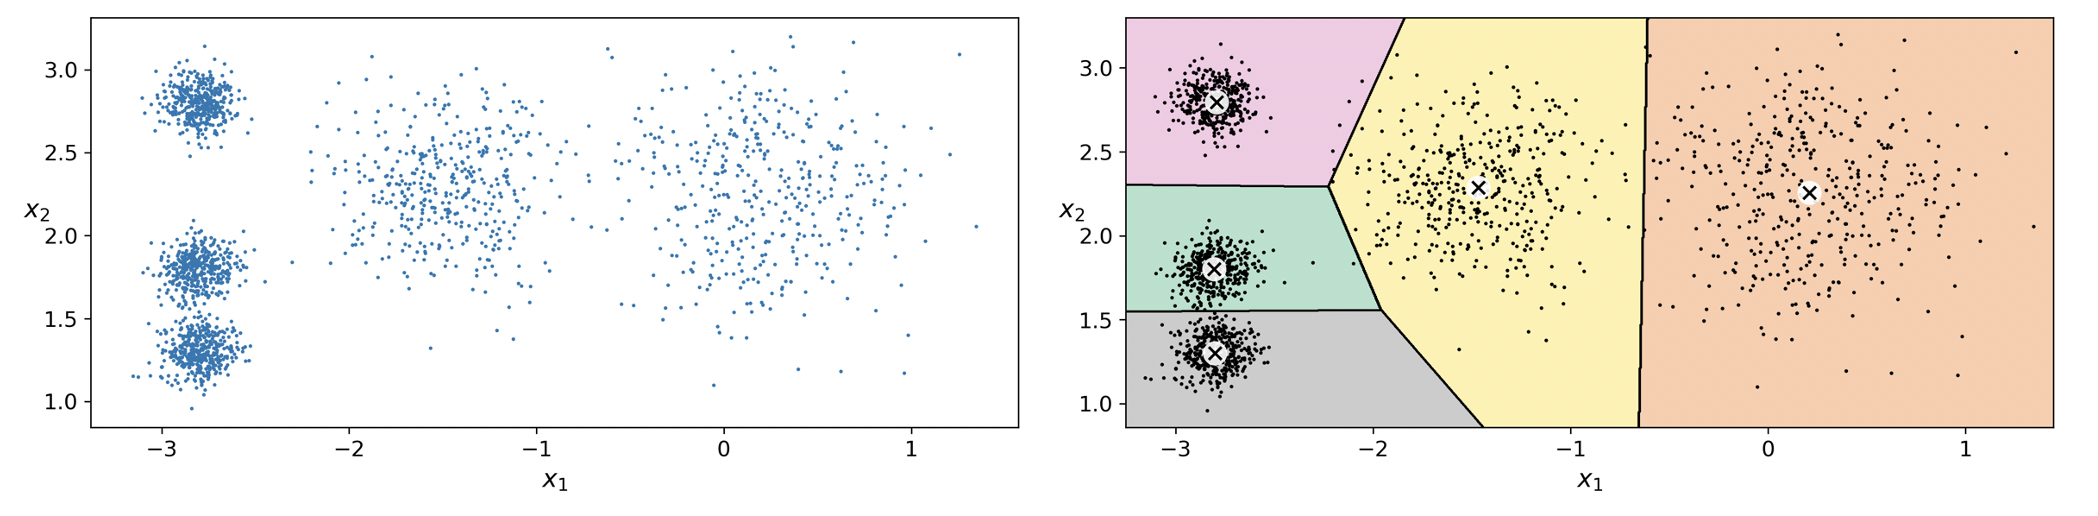
\includegraphics[width=12cm]{graphics/km_example.png}
			\caption{An example of a data distribution and the assigned cluster that k-means has predicted \cite{geron2019hands}.}
			\label{fig:km_handson_example}
		\end{center}
	\end{figure}
	
	This algorithm requires the number of clusters to get specified before initialising the model. The K-means algorithm strives to choose centroids that minimise the inertia, or within-cluster sum-of-squares criterion. The k-means algorithm divides a set of $N$ samples $X$ into $K$ disjoint clusters $C$, each described by the mean $\mu_j$ of the samples in the cluster. The means get commonly called the cluster's "centroids". However, these are not usually points from $X$, although they live in the same space. K-means gets associated with Lloyd's algorithm \cite{geron2019hands, sklearn_km}. 
	
	The algorithm has three steps. The first step chooses the initial centroids, with the most basic method being to choose k samples from the dataset $X$. After initialisation, K-means consists of looping between the two other steps. The first step assigns each sample to its nearest centroid. The second step creates new centroids by taking the mean value of all of the samples assigned to each previous centroid. The difference between the old and the new centroids get computed, and the algorithm iterates these last two steps until this value is less than a threshold. It is, in essence, repeating until the centroids do not move significantly \cite{geron2019hands, sklearn_km}.
	
	K-means scales well to a large number of samples and gets used across a broad range of application areas in many varied fields. K-means is equivalent to the expectation-maximisation algorithm with a small, all-equal, diagonal covariance matrix. When given enough time, K-means will always converge. However, this may be to a local minimum. Converging to a local minimum is highly dependent on the initialisation of the centroids. Therefore, as a result, the computation is often done several times, with different initialisations of the centroids \cite{sklearn_km}.
	
	\subsubsection{Gaussian Mixture Model (GMM)}
	
	A Gaussian mixture model is a probabilistic model that assumes all the data points get generated from a mixture of a finite number of Gaussian distributions with unknown parameters \cite{geron2019hands, sklearn_gmm}. It can get thought of that Gaussian mixture models are a generalised form of k-means clustering to incorporate information about the covariance structure of the data as well as the centres of the underlying Gaussians \cite{sklearn_gmm}. 
	
	There are multiple GMM variants, but in its simplest form for the model to get implemented it requires to know in advance the number of $k$ Gaussian distributions. At the same time, an assumption on the dataset that it gets generated through a probabilistic process (displayed in fig: \ref{fig:gmm_example}) \cite{geron2019hands}. 
	
	\begin{figure}[t]
		\begin{center}
			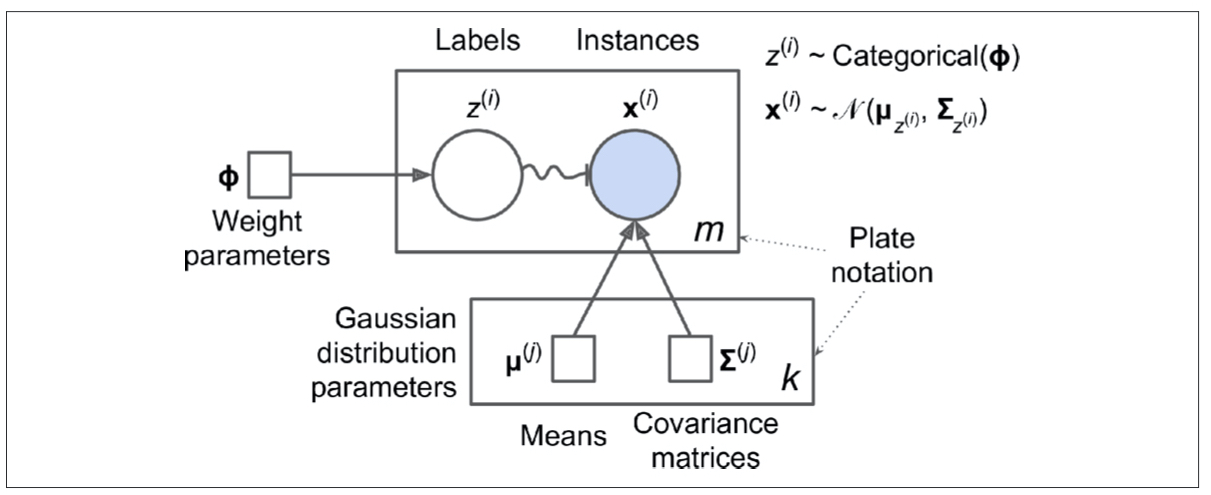
\includegraphics[width=9cm]{graphics/gmm_example.jpeg}
			\caption{An example of a GMM distribution \cite{geron2019hands}.}
			\label{fig:gmm_example}
		\end{center}
	\end{figure}
	
	GMM 's do have many advantages from its speed, and its agnostics, which is due to the algorithm only maximising the likelihood. However, GMM's do have some disadvantages. These are it suffering from singularities. This disadvantage causes the algorithm to diverge and find solutions with infinite likelihoods unless one regularises, which is due to handling of the estimates of the covariance matrices. These become difficult when the algorithm is dealing with insufficiently many points per mixture \cite{sklearn_gmm}. Another disadvantage is the algorithm dealing with several components. This disadvantage is due to the algorithm using all the features it has available. Forcing the need for held-out data to help decide on the number of components required in the absence of external cues \cite{sklearn_gmm}.
	
	\subsubsection{Neural Network (NN)}
	
	Neural Networks (NN) or also known Artificial Neural Networks (ANN), are at the very core of Deep Learning (DL). An ANN is an ML model inspired by networks of biological neurons found in our brains. However, ANN has become very different from their biological cousins that they took inspiration. ANN is what powers Google's image classifications, Apple's Siri and YouTube's video recommendation, as well as learning to beat the worlds best player at the game called Go, named 'DeepMind's Alpha Go' \cite{geron2019hands}.
	
	\subsubsection{Linear Regression}
	%%% Spec
	Linear regression is a model that aims to fit a line of best fit to the data provided \cite{geron2019hands, sklearn_lr}.  A requirement for linear regression is for a set of methods intended for regression in which the target value expects to be a linear combination of the features. In mathematical notation, if $\hat{y}$ is the predicted value. $\hat{y}(w,x)=w_0+w_1x_1+...+w_px_p$
	Across the module, we designate the vector $w=(w_1,...,w_p)$ as the coefficient and w0 as the intercept \cite{sklearn_lr}
	
	LinearRegression fits a linear model with coefficients $w=(w_1,...,w_p)$ to minimise the residual sum of squares between the observed targets in the dataset, and the targets predicted by the linear approximation \cite{sklearn_lr}. To achieve the best fit to the dataset the algorithm chooses the best overall score from the 'Root Mean Square Error' (RMSE). Therefore, to train a linear regression model, we need to find the value of $0$ that minimises the RMSE \cite{geron2019hands}.
	%%%
	Mathematically it solves a problem of the form \cite{sklearn_lr}:
	$\min\limits_{w} = ||Xw-y||^2_2$
	
	The coefficient estimates for linear regression rely on the independence of the features. When features are correlated, and the columns of the design matrix $X$ have an approximate linear dependence, the design matrix becomes close to the singular, which causes the least-squares estimate to become highly sensitive to random errors in the observed target, which in turn produces a large variance. This situation of multicollinearity can arise, for example, when data get collected without an experimental design \cite{sklearn_lr, geron2019hands}.
	
	\subsubsection{Logistic Regression}
	
	%%% Spec
	Logistic regression is an algorithm that gets used for classification and, despite its name, is a linear model rather than a regression one. Logistic regression gets also known in the literature as logit regression, maximum-entropy classification (MaxEnt) or the log-linear classifier. In this model, the probabilities describing the possible outcomes of a single trial getting modelled using a logistic function \cite{sklearn_lr, handson_book}. Logistic regression's model estimated probability in its vectorised form: $\hat{p}=h_\theta(x) = \sigma(x^T\theta)$ \cite{geron2019hands}.
	
	\begin{figure}[t]
		\begin{center}
			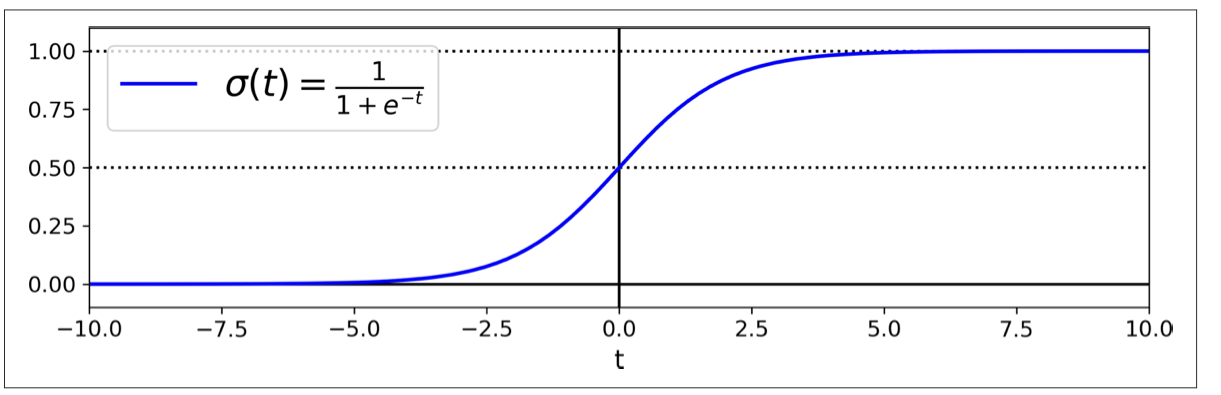
\includegraphics[width=9cm]{graphics/logistic_reg.jpeg}
			\caption{An example of a logistic regression threshold distribution \cite{geron2019hands}.}
			\label{fig:logr_example}
		\end{center}
		
	\end{figure}
	
	Logistic regression gets used to estimate the probability that an instance belongs to a particular class. If the estimated probability is greater than 50\%, the model predicts that the instance belongs to that class. If the model has predicted that the instance belongs to that class, also known as the positive class, it gets a '1' label  (see fig \ref{fig:logr_example}) \cite{geron2019hands}. Logistic regression can fit binary, One-vs-Rest, or multinomial logistic regression. That also has an optional $\ell1, \ell2$ or Elastic-Net regularisation \cite{sklearn_lr}.
	
	\subsubsection{Support Vector Machines (SVM)}
	%%% Spec
	Support Vector Machine (SVM) is a powerful and versatile ML model. The model is capable of performing linear or nonlinear classification, regression and even outlier detection \cite{geron2019hands, sklearn_svm}. This model is one of the most popular ML models and is best suited for small to medium-sized datasets. The model aims to separate the data categories by using a decision boundary, with the largest margin between them. Due to the model using a large margin to separate the data, the algorithm gets known as the 'large margin classification' \cite{geron2019hands}.
	%%%
	
	SVMs are a set of supervised learning methods and have many advantages, especially when working in high dimensional spaces. SVMs are also useful in situations where the number of dimensions is greater than the number of samples. Due to the model using subsets of the training points in the decision function, the model is memory efficient, and it is very versatile. The model is very versatile due to the different kernel functions are can be used \cite{sklearn_svm}. Although the model does have many strengths, it does also have a few disadvantages. A disadvantage is if the number of features is considerably greater than the number of data samples, then overfitting can happen. A way to overcome this is to choose different kernel functions, and regularisation of the term is crucial. Another disadvantage is that SVMs do not provide probability estimates. These estimates get calculated by using an expensive five-fold cross-validation \cite{sklearn_svm}.

	
	\subsubsection{k-Nearest Neighbour (kNN)}
		\label{seb_sec:kNN}
		
		A Neighbours-based classification is a type of instance-based learning or non-generalising learning: it does not attempt to construct a general internal model, but simply stores instances of the training data. Classification gets computed from a simple majority vote of the nearest neighbours of each point: a query point is assigned the data class which has the most representatives within the nearest neighbours of the point. Although kNN gets usually used as a classification method, it can also get used as a regression method.
		
		The k-neighbours classification in KNeighborsClassifier is the most commonly used technique. The optimal choice of the value k is highly data-dependent: in general, a larger k suppresses the effects of noise but makes the classification boundaries less distinct \cite{sklearn_knn}.
		
	\subsection{Dimensionality Reduction}
		\label{seb_sec:dd}
		
		Dimensionality reduction, or dimension reduction, is the transformation of data from a high-dimensional space into a low-dimensional space so that the low-dimensional representation retains some meaningful properties of the original data, ideally close to its intrinsic dimension \cite{geron2019hands}.
		
		Dimensionality reduction aims to reduce the dimensionality of the data. However, it also strives to maintain the meaningfulness of the data fundamentally at the same time \cite{bishop2006pattern}. The idea is to find a low dimensionality of the data but a useful representation of it. The process of dimensionality reduction is to discover the intrinsic dimensionality of the data. This reduction gets used due to some high dimensionality data actually being very low in dimensionality in reality.
		
		Dimensionality reduction aims to reduce the curse of dimensionality. The curse of dimensionality refers to various phenomena that arise when analysing and organising data in high-dimensional spaces that do not occur in low-dimensional settings such as the three-dimensional physical space of everyday experience. The expression was coined by Richard E. Bellman when considering problems in dynamic programming \cite{bishop2006pattern}.
		
		The cursed of dimensionally phenomena usually occurs in: numerical analysis, sampling, combinatorics, machine learning, data mining and databases. The common theme of these problems is that when the dimensionality increases, the volume of the space increases so fast that the available data becomes sparse. This sparsity is problematic for any method that requires statistical significance. To obtain a statistically sound and reliable result, the amount of data needed to support the result often grows exponentially with the dimensionality. Also, organising and searching data relies on detecting areas, within the data, where objects form groups with similar properties, for example, in high dimensional data. However, all objects appear to be sparse and dissimilar in many ways, which prevents common data organisation strategies from being efficient \cite{geron2019hands}.
		
		In a nutshell, the efficiency of many algorithms depends on the number of dimensions. However, datasets can hold a lot of redundant features. For example, not all words are useful in classifying documents like: and, or, the, of. Distance-based similarity algorithms, like K-Means and GMM, are at least linear to the number of dimensions. High dimensionality is very expensive to store, and indexing and retrieving data in high dimensional space is difficult.
	
		Principal Component Analysis (PCA) is a prevalent data reduction algorithm that gets classed as an unsupervised method. 
		
		PCA is a linear method used which will aim to reduce the data's dimensionality. It aims to do this by removing the interrelated variables while retaining as much as possible. The algorithm seeks to keeping as much variation as possible that is present within the data set.
		
		The dimensionality reduction gets achieved by transforming the data into a new set of variables. These new variables are called the principal components (PCs). These PCs are uncorrelated and get ordered in a way that the first couple of PCs retains the most amount of the variation that is present in the original variables.
		
		PCA is a decorrelation method which will linearly transform the data so that covariance values are all zeros, which, as a result, retains the components with the largest variances. While also getting rid of the components that have small variance, therefore achieving dimensionality reduction. The Eigenvectors (more below) correspond to the different principal components \cite{friedman2001elements}. 
	
	\subsection{Machine Learning in Education}
		\label{seb_sec:ml_in_learning}
	
	We will look at the styles and way machine learning gets currently taught to help people learn the different aspects of machine learning and in most cases, the overall characteristics of data science. we will be looking at classical approaches as well at any modern-day style teaching or machine learning educational games available. 
	
	\subsubsection{Classical Approaches}
		\label{sub_sec:classical_teach_learn}
		
		We have used the term, 'classical approach', to define methods of teaching and learning that get done in a way that is similar to what would get traditionally expected in a classroom.  Although taking into account modern takes on this approach in the forms of delivery. The classical approach is what we classify teaching and learning that gets based on a here is the knowledge, here is a task and here is the solution. Now onto the next problem, for example.
		
		Some of the most popular ways of learning machine learning concepts without going to university are through online learning platforms like Udemy, Coursera, edX and youTube, or you have your traditional style of lectures usually found at universities.
		
		Udemy claims to be "Improving Lives Through Learning \cite{udemy}". Udemy claims that they are the leading global marketplace for teaching and learning, having connected millions of students to skills that are needed to succeed. They have 35m learners enrolled in courses, 57k instructors, 130k courses on offer, 400m course enrollments, 110m minutes of video, 65+ languages available, over 7k Enterprise customers and they claim that 80\% of the fortune 100 companies trust them for employee upskilling \cite{udemy}. Udemy also claims that they have helped all different kinds of organisations to prepare for the ever-changing world of work. Udemy's "curated collection of top-rated business and technical courses gives companies, governments, and nonprofits the power to develop in-house expertise and satisfy employees' hunger for learning and development \cite{udemy}." 
		
		Coursera, another online teaching and learning platform, "envision a world where anyone, anywhere can transform their life by accessing the world's best learning experience \cite{coursera}." Coursera claim that you can "gain a job-relevant skill in under 2 hours" by enrolling in Guided Projects to learn job-relevant skills and industry tools. Guided Projects require a smaller time commitment, and provide practice using tools in real-world scenarios, so you can build the job skills you need, right when you need them but if you want to master a subject, it will take 4 - 6 months \cite{coursera}. Coursera are also moving in the space of online degrees. Transform your career with a degree online from a world-class university on Coursera. Our modular degree learning experience gives you the ability to study on your own schedule and earn credit as you complete your course assignments. 
		
		youTube videos can be a powerful educational and motivational tool. However, a great deal of the medium's power lies not in itself but in how it gets used. Video is not an end in itself, but a means toward achieving learning goals and objectives. Educators are increasingly using YouTube as a pedagogic resource for everything. Guidelines recommended by Clark and Mayer \cite{clark2016learning} suggest the appropriate use of any media improve learning. Suggestion means that media must get aligned with expected learning or performance outcome, reduce cognitive load, exclude simple text or graphics, be appropriate for target learner's learning literacy's Educators (and students alike). Through doing this will find that video is a significant catalyst and facilitator for classroom discourse and analysis \cite{duffy2008engaging}.
		
		While these are all popular and effective methods of teaching and learning, these methods are all purpose-driven with the content and resources getting created to deliver to the student a key concept and then moving on. This issue can get exacerbated, especially in the case of youTube, the way tutorials and lessons can get created can get very disjointed. In some cases, with different content creators teaching the same content but in different ways, can be very confusing for the learner. However, although these forms of e-learning can be beneficial, they never genuinely allowing the student to be able to just play around with learning content. Not allowing the learns to experiment with what happens if they do this or if they do that and physically see it happening, especially at a novice level. In a way, it is like a conveyer belt, everything moving along to the next thing, or in the case of learning, the next topic.
		
		Although these methods are, in their own right, all good ways to learn, they all, in essence, tell the learner here is the content and this is what it does. These methods have no way for the learner to be able just deep dive into the models and interact with them, and in most cases will only have a one use case model implemented that has minimal interaction. Therefore relying on the learner to go away and learn more about the models and then manually tweak them.
		
	
	\subsubsection{Machine Learning Edu-Games}
		\label{sub_sec:ml_edu_games}
		
		Most of the focus, in regards to ML within education, is on ML getting used to aid educational purposes, like predicting students grades, improving student retention, testing students and predicting student performance \cite{kuvcak2018machine}, rather than getting used to enable the learning and teach its concepts, especially in a Serious game context.
	
	\section{Proposed Solution}
	% Taken from spec
	The overall aim of the proposed solution is to create a fun, educating game about ML. The players will be, at the core of the solution, playing a game that interacts with different ML models. The player(s) will be manipulating the game board and data points to affect the decision boundary, or to figure out where the decision boundary or centre of the cluster is. The solution will get created by using  Pygame and will have many different algorithms in the background, doing the main game mechanics, through using libraries like SKLearn \cite{sklearn_api} and Tensorflow \cite{tensorflow2015-whitepaper}.
	
	\section{Summary and Overview of Proposed Solution}
		We have found that educational games, although they can take many forms, can only be described as so only if the games that get designed aim to help learners learn. The learning can involve certain subjects, expand concepts, reinforce development, understand a historical event or culture, or assist them in learning a skill as they play the game. Also, we have found out that a technique used to motivate plays, through extrinsic means, to behave in a certain way is called gamification. Gamification is a powerful and useful tool when implemented correctly. It is so good that it gets used almost all the time within a whole array of application. There is also a method of gamification explicitly aimed at the field of science and its wide variety of topics. This version of gamification is known as serious games. These types of gamification require the user to be able to explore and interact with the data that is on offer throughout the game. Promoting a sense of exploring and discovery.
		
		Machine learning is a toolbox that consists of two primary methods. These methods are known as supervised and unsupervised learning. Supervised learning is when the model uses the target, also known as label, data. These allow the models to check how well they fit the data and its predictions based on the actual expected outcome of the data's target. The main goal of supervised learning is usually to do one of two things, either regression or classification. These supervised methods include linear regression, logistic regression and neural networks.
		
		In comparison, unsupervised learning's models expect there to be no labels to the data. So the models will fit and predict the data based on the model selected actions. These actions can be clustering, data association and dimensionality reduction. Some of these algorithms include k-means, PCA.
		
		The proposed solution will aim to create an application that will incorporate elements of gamification and serious games, as well as actual gaming mechanics to create a fun and engaging game. This game will be about machine learning while providing aspects of teaching and learning. The teaching and learning will be in the form of learning reading content, quizzes and exploration through the game by interacting with the models.